% Heterodyne laser interferometer: reference and measurement paths
\documentclass[dvisvgm,tikz,border=4pt]{standalone}
% Shared preamble for the TikZ figures in images-1/src (compiled by build.sh)
\usepackage{helvet}
\renewcommand\familydefault{\sfdefault}
\usepackage{amsmath, amssymb}
\usetikzlibrary{arrows.meta, calc, decorations.pathreplacing, patterns, positioning, shapes.geometric, 3d, perspective, fit, backgrounds}
% palette shared with slides.scss and the Graphviz diagrams
\definecolor{dmred}{HTML}{880000}
\definecolor{dmblue}{HTML}{000088}
\definecolor{dmgreen}{HTML}{008800}
\definecolor{dmorange}{HTML}{E08A1E}
\definecolor{ink}{HTML}{333333}
\definecolor{fillblue}{HTML}{E8E8F8}
\definecolor{fillred}{HTML}{F3EAEA}
\definecolor{fillgreen}{HTML}{E8F4E8}
\definecolor{fillorange}{HTML}{FDF0DC}
\definecolor{steel}{HTML}{C9D3DC}
\definecolor{steeldk}{HTML}{8FA3B5}
\definecolor{metal}{HTML}{D9D9D9}
\definecolor{metaldk}{HTML}{A6A6A6}
\tikzset{
  >={Stealth[length=7pt]},
  every picture/.style={line cap=round, line join=round, font=\large},
  proj/.style={gray, dashed, thin},
  dim/.style={<->, >={Stealth[length=5pt]}, thin},
  ext/.style={very thin, gray},
  callout/.style={gray!70!black, thin},
  % datum (origin) symbol
  % pics use absolute sizes so they look the same in mm-scaled drawings
  datum/.pic={
    \fill[white] (0,0) circle (0.22cm);
    \fill[black] (0,0) -- ++(0.22cm,0) arc[start angle=0, end angle=-90, radius=0.22cm] -- cycle;
    \fill[black] (0,0) -- ++(-0.22cm,0) arc[start angle=180, end angle=90, radius=0.22cm] -- cycle;
    \draw[thick] (0,0) circle (0.22cm);
  },
  % reference symbols (absolute sizes): origins have a double circle with a filled quadrant
  wporigin/.pic={
    \draw[thick, fill=white] (0,0) circle (0.3cm);
    \fill[black] (0,0) -- (0.18cm,0) arc[start angle=0, end angle=-90, radius=0.18cm] -- cycle;
    \draw[thick] (0,0) circle (0.18cm);
    \draw (-0.3cm,0) -- (0.3cm,0) (0,-0.3cm) -- (0,0.3cm);
  },
  machorigin/.pic={
    \draw[thick, fill=white] (0,0) circle (0.3cm);
    \fill[black] (0,0) -- (-0.18cm,0) arc[start angle=180, end angle=90, radius=0.18cm] -- cycle;
    \draw[thick] (0,0) circle (0.18cm);
    \draw (-0.3cm,0) -- (0.3cm,0) (0,-0.3cm) -- (0,0.3cm);
  },
  supportpt/.pic={
    \draw[thick, fill=white] (0,0) circle (0.15cm);
    \draw (-0.15cm,0) -- (0.15cm,0) (0,-0.15cm) -- (0,0.15cm);
  },
  regpt/.pic={
    \draw[thick, fill=white] (0,0) circle (0.24cm);
    \draw[thick] (0,0) circle (0.15cm);
    \draw (-0.15cm,0) -- (0.15cm,0) (0,-0.15cm) -- (0,0.15cm);
  },
  % support / registration point (generic)
  target/.pic={
    \draw[thick, fill=white] (0,0) circle (0.12cm);
    \draw (-0.2cm,0) -- (0.2cm,0) (0,-0.2cm) -- (0,0.2cm);
  },
}

\begin{document}
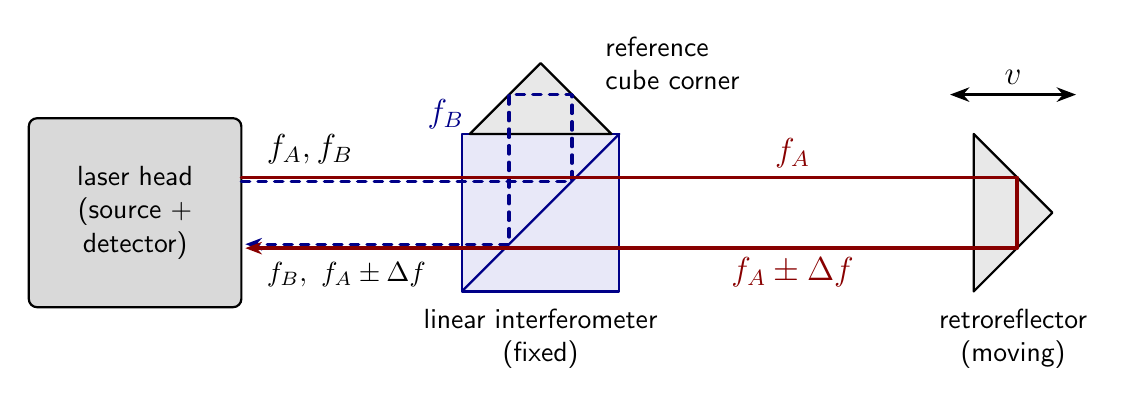
\begin{tikzpicture}[font=\large]
  \tikzset{beamA/.style={dmred, very thick, -{Stealth[length=6pt]}},
           beamB/.style={dmblue, very thick, dashed, -{Stealth[length=6pt]}}}
  % laser head: two frequencies out, detector in
  \draw[thick, fill=metal, rounded corners=3pt] (-1.5,-1.2) rectangle (1.2,1.2);
  \node[align=center, font=\normalsize] at (-0.15,0) {laser head\\(source +\\detector)};
  % polarizing beam splitter (fixed interferometer) and reference cube corner
  \draw[thick, fill=fillblue, draw=dmblue] (4,-1) rectangle (6,1);
  \draw[thick, dmblue] (4,-1) -- (6,1);
  % 90-degree corner: mirrors y = 1.9 -/+ (x - 5); beam corners on them
  \draw[thick, fill=metal!60] (4.1,1) -- (5,1.9) -- (5.9,1) -- cycle;
  \node[anchor=west, align=left, font=\normalsize] at (5.7,1.9) {reference\\cube corner};
  \node[below, align=center, font=\normalsize] at (5,-1.1) {linear interferometer\\(fixed)};
  % moving retroreflector
  \begin{scope}[shift={(10.5,0)}]
    % 90-degree corner: mirrors x = 1 -/+ y; beam corners on them
    \draw[thick, fill=metal!60] (0,-1) -- (1,0) -- (0,1) -- cycle;
    \node[below, align=center, font=\normalsize] at (0.5,-1.1) {retroreflector\\(moving)};
    \draw[<->, thick] (-0.3,1.5) -- node[above] {$v$} (1.3,1.5);
  \end{scope}
  % f_B: reflected by the splitter into the reference corner and back
  \draw[beamB] (1.2,0.4) -- (5.4,0.4) -- (5.4,1.5) -- (4.6,1.5) -- (4.6,-0.4) -- (1.25,-0.4);
  % f_A: through the splitter to the moving retroreflector and back, Doppler shifted
  \draw[beamA] (1.2,0.45) -- (10.5,0.45) -- (11.05,0.45) -- (11.05,-0.45) -- (1.25,-0.45);
  \node[dmred, above] at (8.2,0.45) {$f_A$};
  \node[dmred, below] at (8.2,-0.45) {$f_A \pm \Delta f$};
  \node[anchor=south west] at (1.4,0.5) {$f_A, f_B$};
  \node[anchor=north west, font=\normalsize] at (1.4,-0.5) {$f_B,\ f_A \pm \Delta f$};
  \node[dmblue, left] at (4.15,1.25) {$f_B$};
\end{tikzpicture}
\end{document}
